%\documentclass[10pt,a4paper]{IEEEtran}
%\usepackage[latin1]{inputenc}
%\usepackage{amsmath}
%\usepackage{amsfonts}
%\usepackage{amssymb}
%\usepackage{graphicx}
%\begin{document}

Nosso objetivo principal neste trabalho é estimar a função $\mathcal{Q}_{y_t|y_{t-p}}^\alpha(t)$ que corresponde ao quantil $\alpha$ quando previsto $p$ passos à frente, para uma dada série temporal $y_t$, como a apresentada na figura \ref{fig:exemployt}. Então, dada uma sequência $\{y_t\}$, podemos fazer uma correspondência entre cada observação $y_t$ e sua defasagem de ordem $p$. A figura \ref{fig:exemploar} mostra um exemplo dessa relação. 

\begin{figure}[h]
\centering
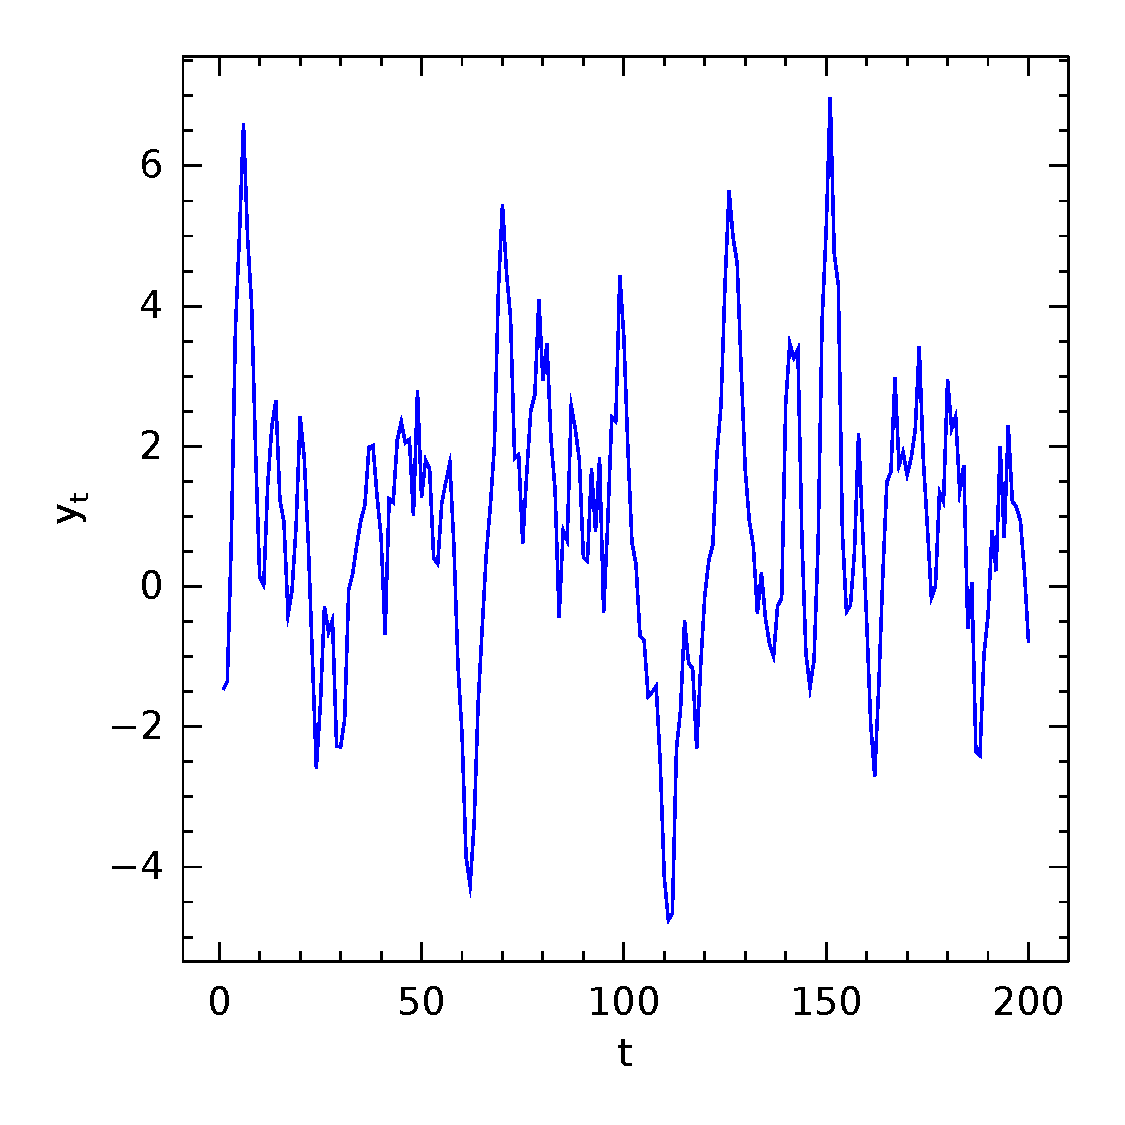
\includegraphics[width=0.7\linewidth]{Figuras/exemplo-yt}
\caption{Série temporal $y_t$}
\label{fig:exemployt}
\end{figure}

\begin{figure}[h]
\centering
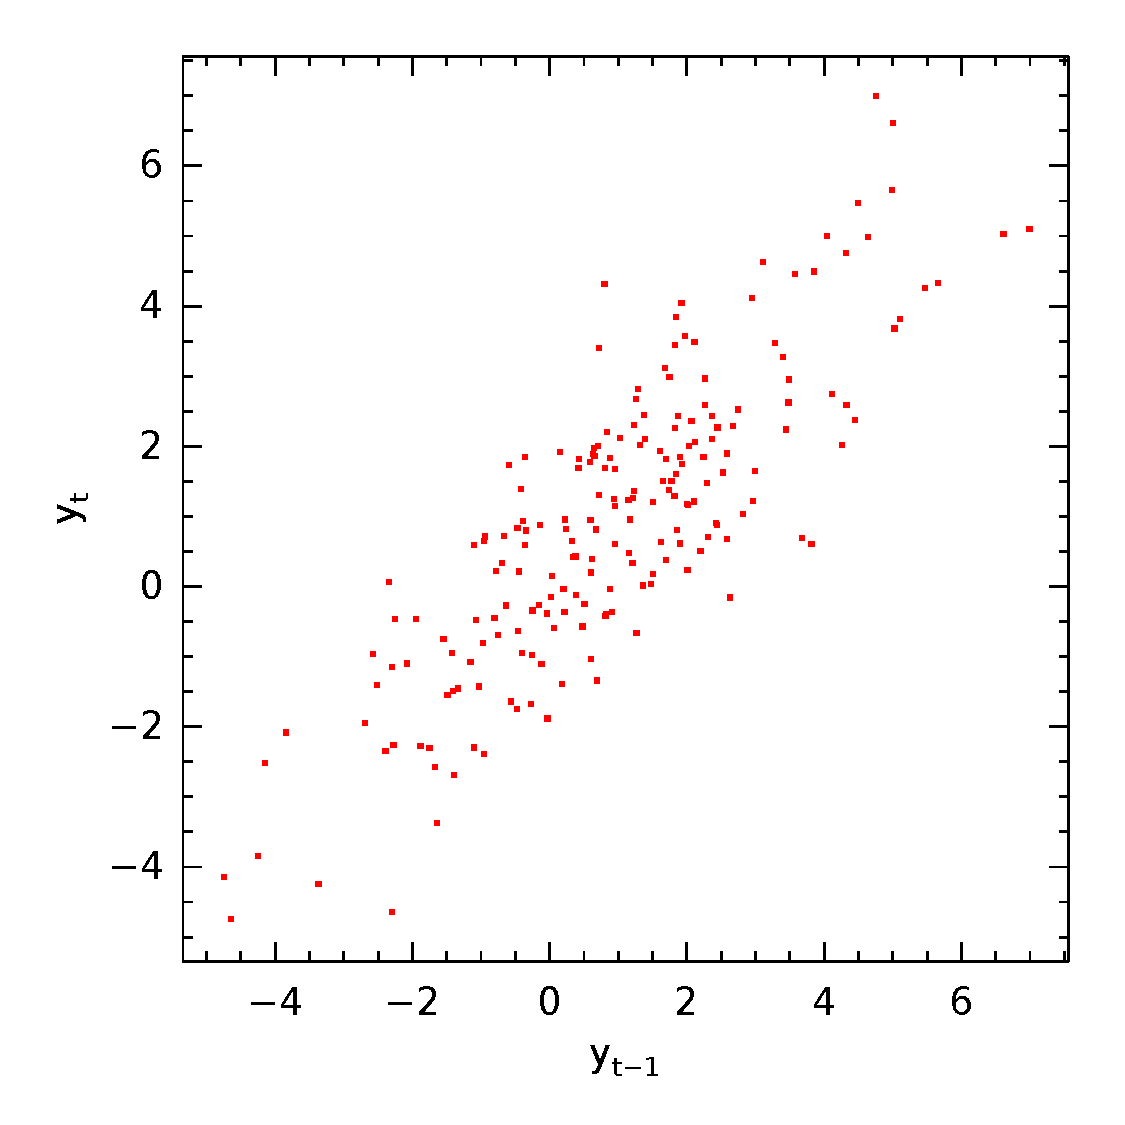
\includegraphics[width=0.7\linewidth]{Figuras/exemplo-ar}
\caption[Tst]{Relationship between $y_t$ and its first lag $y_{t-1}$}
\label{fig:exemploar}
\end{figure}

\todo[inline]{Refazer gráfico com pontos maiores}

Vamos investigar duas maneiras de estimar os quantis da relação acima: utilizando um modelo linear e um modelo não paramétrico.


\section{Estimando a QAR com um modelo linear}

Ao estimar um modelo de regressão quantílica, estamos interessados em encontrar uma função $f$ que minimize a soma dos erros
\begin{equation}
\min_{f}\sum_{i=1}^{n}\alpha|y_{t}-f(t)|^{+}+(1-\alpha)|y_{t}-f(t)|^{-},
\end{equation}
em que $|x|^+=\max\{0,x\}$ e $|x|^-=-\min\{0,x\}$.
Para resolver este problema como um problema de programação linear, podemos criar variáveis $\delta^+$ e $\delta^-$ para representar as funções $|\cdot|^+$ e $|\cdot|^-$, respectivamente, e montá-lo da seguinte forma:
\begin{equation}
\begin{aligned}\min_{f} & \sum_{i=1}^{n}\left(\lambda\delta_{i}^{+}+(1-\lambda)\delta_{i}^{-}\right)\\
\mbox{sujeito à } & \delta_{i}^{+}-\delta_{i}^{-}=y_{i}-f(x_{i}),\qquad\forall i\in\{1,\dots,n\},\\
& \delta_i^+,\delta_i^- \geq 0, \qquad \forall \{1,\dots,n\}.
\end{aligned}
\end{equation}

Quando assumimos que a função $f$ que estima o $\alpha$-ésimo quantil é uma função linear, tal que $f(x) = \beta_0 + \beta^T x$, os valores de $\beta_0$ e $\beta$ podem ser obtidos como sendo aqueles vindos da solução do seguinte problema de minimização:
\begin{equation}
\begin{aligned}\min_{\beta_0,\beta} & \sum_{i=1}^{n}\left(\alpha\delta_{i}^{+}+(1-\alpha)\delta_{i}^{-}\right)\\
\mbox{sujeito � } & \delta_{i}^{+}-\delta_{i}^{-}=y_{i} - \beta_0 - \beta^T x_{i},\qquad\forall i\in\{1,\dots,n\},\\
& \delta_i^+,\delta_i^- \geq 0, \qquad \forall \{1,\dots,n\}.
\end{aligned}
\end{equation}

%Utilizando um modelo linear de regressão quantílica para estimar os coeficientes do QAR %

\todo[inline]{Resultados para a estimação linear}

\section{Estimando a QAR não parametricamente}

Fitting a linear estimator for the Quantile Auto Regression isn't appropriate  when nonlinearity is present in the data. This nonlinearity may produce a linear estimator that underestimates the quantile for a chunk of data while overestimating for the other chunk (we illustrate this in figure \ref{fig:nonlinear}). To prevent this issue from occurring we propose a modification which we let the prediction $\mathcal{Q}_{y_t|y_{t-1}}^\alpha(t)$ adjust freely to the data and its nonlinearities. To prevent overfitting and smoothen our predictor, we include a penalty on its roughness by including the $\ell_1$ norm of its second derivative. For more information on the $\ell_1$ norm acting as a filter, one can refer to \cite{kim2009ell_1}.

\begin{figure}
\centering
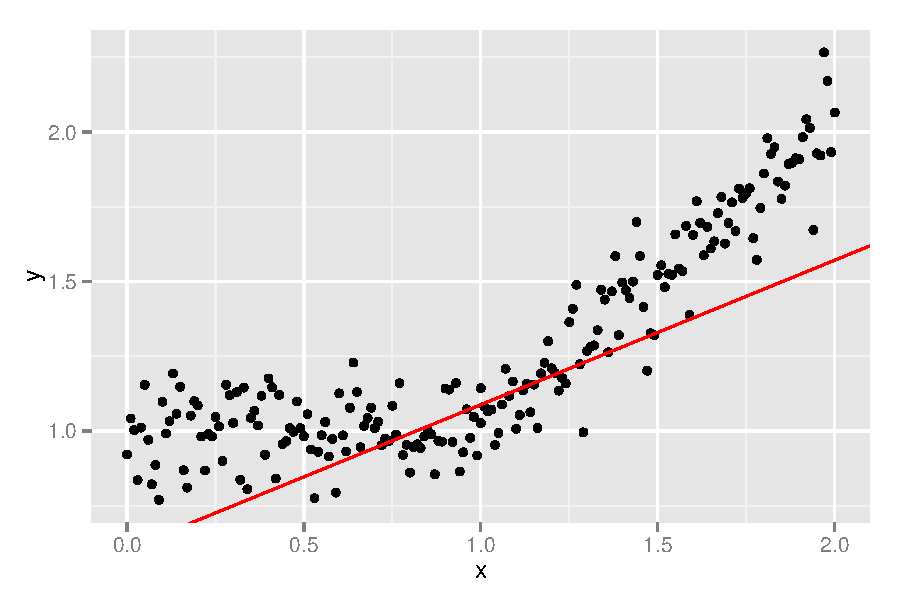
\includegraphics[width=0.7\linewidth]{../Paper_IEEE/nonlinear}
\caption{Example of data where nonlinearity is present and a linear quantile estimator is employed}
\label{fig:nonlinear}
\end{figure}


% notação estatística de ordem. com x^(0)

Let $\{\tilde{y}_t \}_{t=1}^n$ be the sequence of observations in time $t$. Now, let $\tilde{x}_t$ be the $p-$lagged time series of $\tilde{y}_t$, such that $\tilde{x}_t = L^p(\tilde{y}_t)$, where $L$ is the lag operator. Matching each observation $\tilde{y}_t$ with its $p-$lagged correspondent $\tilde{x}_t$ will produce $n-p$ pairs $\{(\tilde{y}_t,\tilde{x}_t)\}_{t=p+1}^n$ (note that the first $p$ observations of $y_t$ must be discarded). When we order the observation of $x$ in such way that they are in growing order
$$\tilde{x}_{(p+1)} \leq \tilde{x}_{(p+2)} \leq \dots \leq \tilde{x}_{(n)},$$ 
we can then define $\{x_i\}_{i=1}^{n-p} = \{\tilde{x}_{(t)} \}_{t=p+1}^{n}$ and $\{y_i\}_{i=1}^{n-p} = \{\tilde{y}_{(t)} \}_{t=p+1}^{n}$ and $I = \{2,\dots, n-p-1\}$. As we need the second difference of $q_i$, $I$ has to be shortened by two elements.

Our optimization model to estimate the nonparametric quantile is as follows:
\begin{equation}
\begin{split}
\mathcal{Q}_{y_t|y_{t-1}}^\alpha(i) =\underset{q_{i}}{\arg\min}\sum_{i\in I}\left(|y_{i}-q_{i}|^{+}\alpha + |y_{i}-q_{i}|^{-}(1-\alpha)\right) \\ +\lambda  \sum_{i\in I}|D^{2}q_{i}|,
\end{split}
\end{equation}
where $D^2 q_t$ is the second derivative of the $q_t$ function, calculated as follows:
\begin{equation*}
D^{2}q_{i}=\left(\frac{q_{i+1}-q_{i}}{x_{i+1}-x_{i}}\right)-\left(\frac{q_{i}-q_{i-1}}{x_{i}-x_{i-1}}\right).
\end{equation*}
The first part on the objective function is the usual quantile regression condition for $\{q_i\}$. The second part is the $\ell_1$-filter. The purpose of a filter is to control the amount of variation for our estimator $q_i$. When no penalty is employed we would always get $q_i = y_i$. On the other hand, when $\lambda \rightarrow \infty$, our estimator approaches the linear quantile regression.

The output of our optimization problem is a sequence of ordered points $\{(x_i, q_i)\}_{i \in I}$. The next step is to interpolate these points in order to provide an estimation for any other value of x. To address this issue, we propose a B-splines interpolation, that will be discussed in another subsection.

When estimating quantiles for a few different values of $\alpha$, however, sometimes we find them overlapping each other, which we call crossing quantiles. To prevent this, we include a non-crossing constraint:
\begin{equation}
q_i^{\alpha} \leq q_i^{\alpha'}, \quad \forall i \in I, \alpha < \alpha'.
\label{eq:non-crossing}
\end{equation} 

\todo[inline]{traduzir trecho acima}

Testamos a regressão quantílica não paramétrica para estimar quantis para diversos tipos de dados e de penalizações. A seguir, apresentamos o resultado da regressão quantílica para dados gerados a partir de um modelo ARIMA com diversos valores distintos de penalização, com ou sem a restrição de não-cruzamento de quantis. As figuras contém todos os quantis entre 1\% e 99\%.

\begin{figure}
\centering
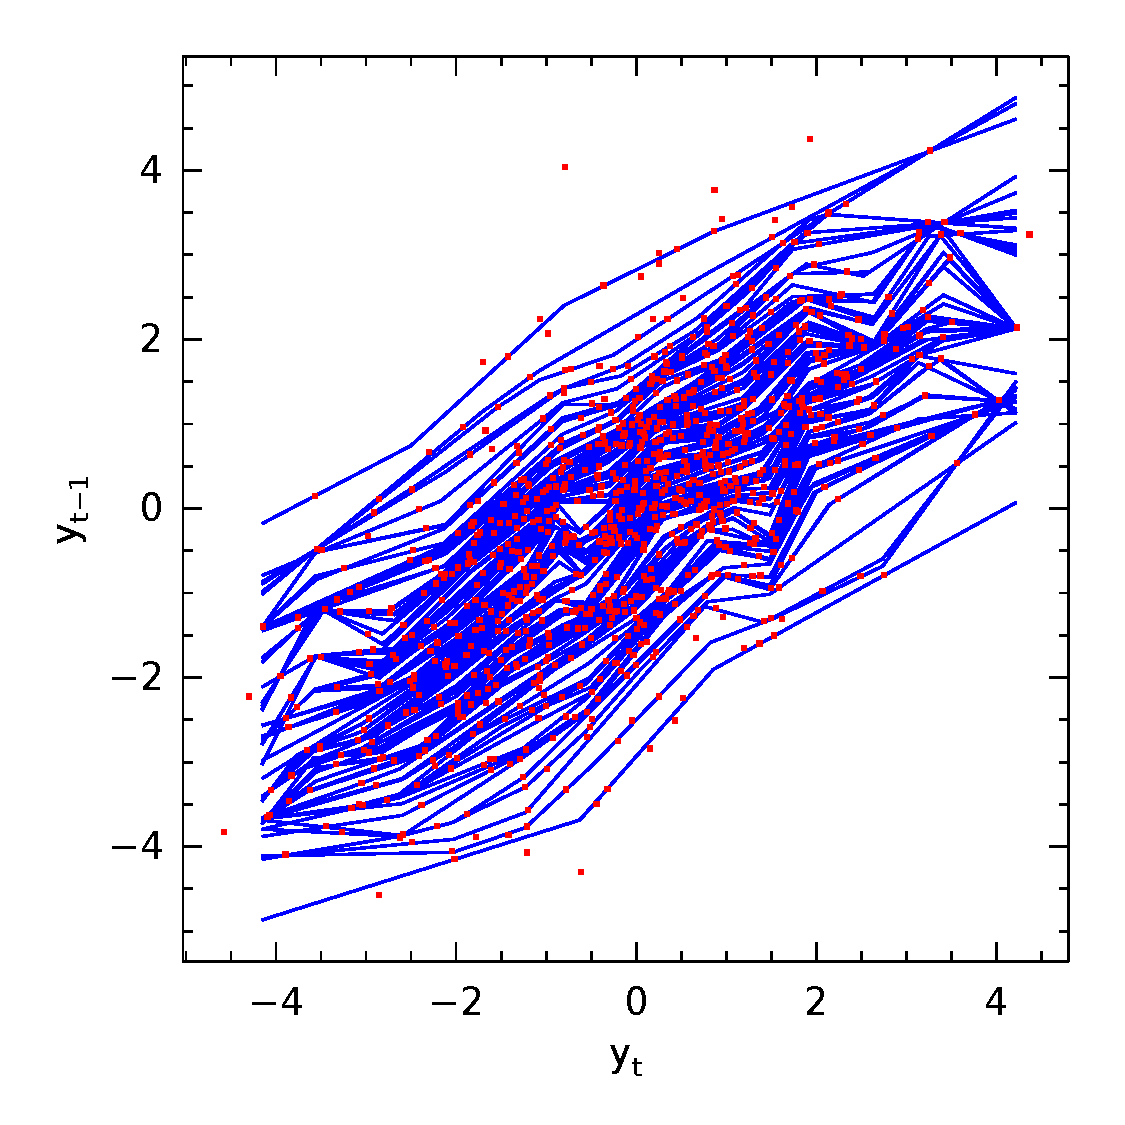
\includegraphics[width=0.6\linewidth]{Figuras/arima-crossing-03.pdf}
\caption{Dados simulados ARIMA com penalização $\lambda=0.3$}
\label{fig:arima-crossing-03}
\end{figure}

\begin{figure}
\centering
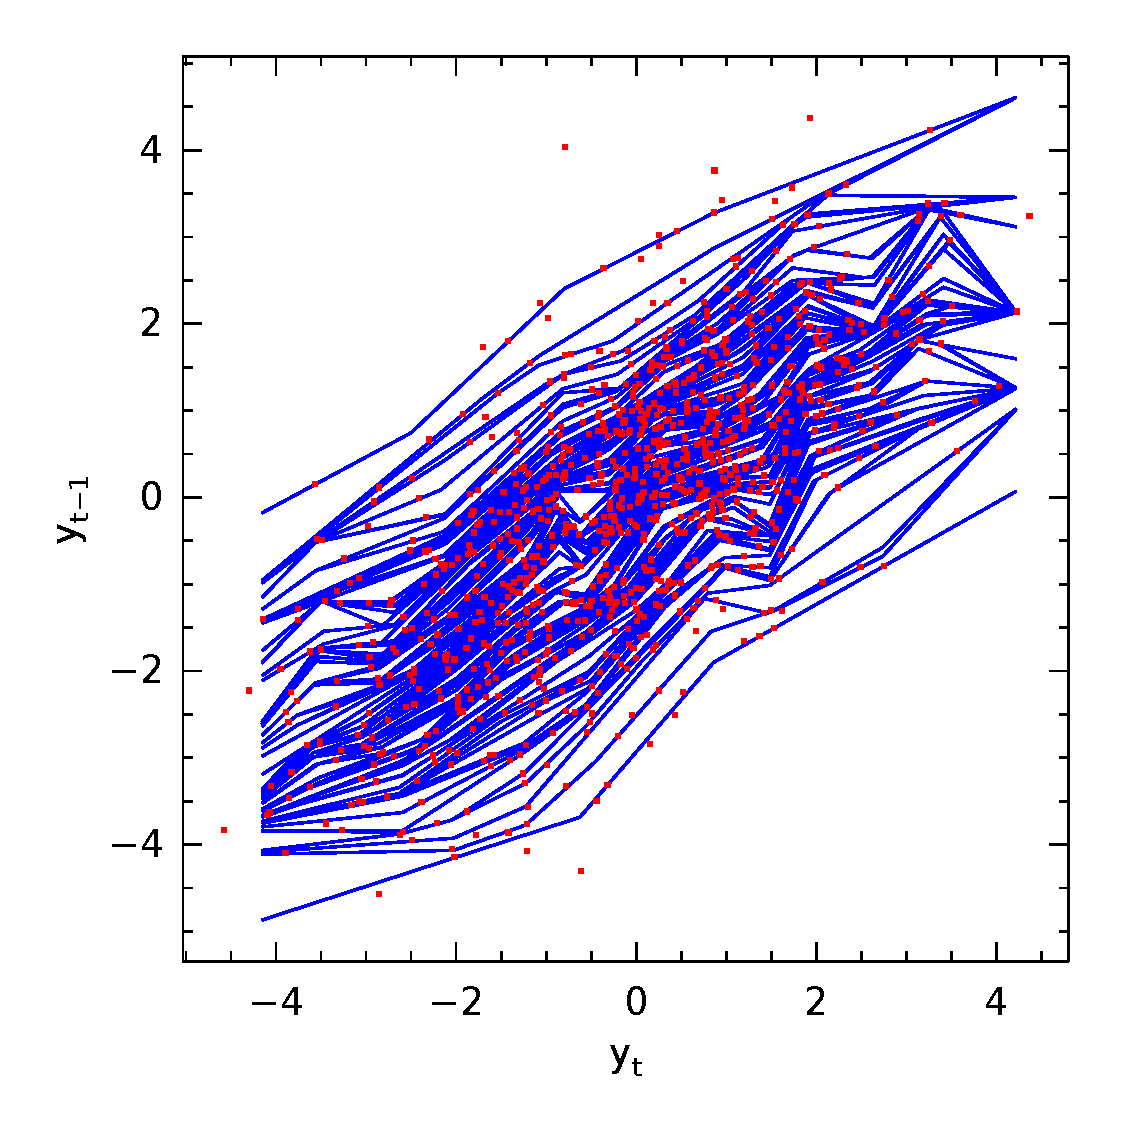
\includegraphics[width=0.5\linewidth]{Figuras/arima-noncrossing-03.pdf}
\caption{Dados simulados ARIMA com penalização $\lambda=0.3$ e restrição de não cruzamento de quantis}
\label{fig:arima-noncrossing-03}
\end{figure}

\begin{figure}
\centering
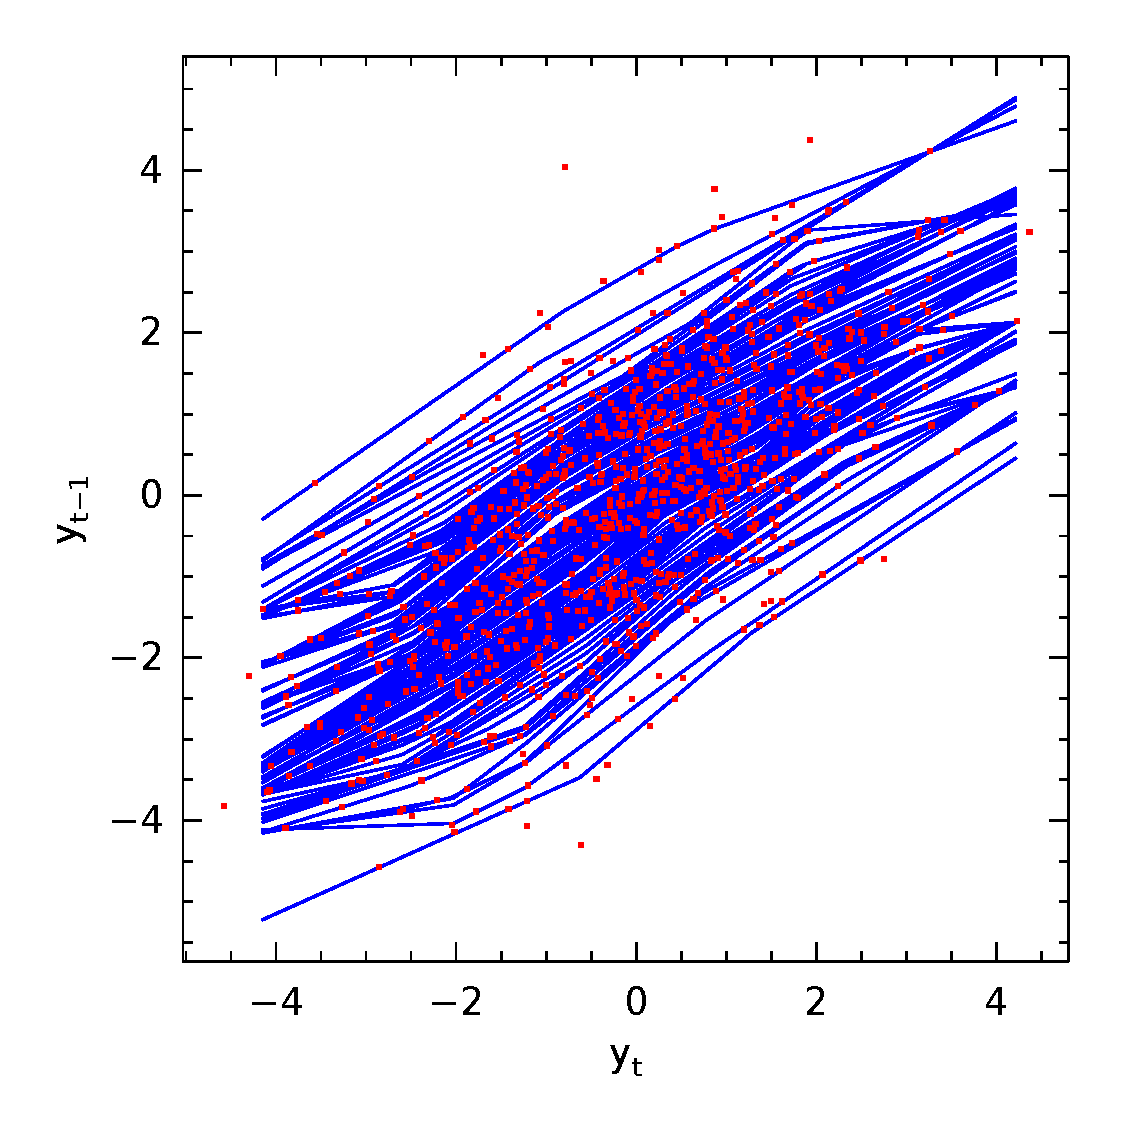
\includegraphics[width=0.6\linewidth]{Figuras/arima-crossing-1.pdf}
\caption{Dados simulados ARIMA com penalização $\lambda=1$}
\label{fig:arima-crossing-1}
\end{figure}

\begin{figure}
\centering
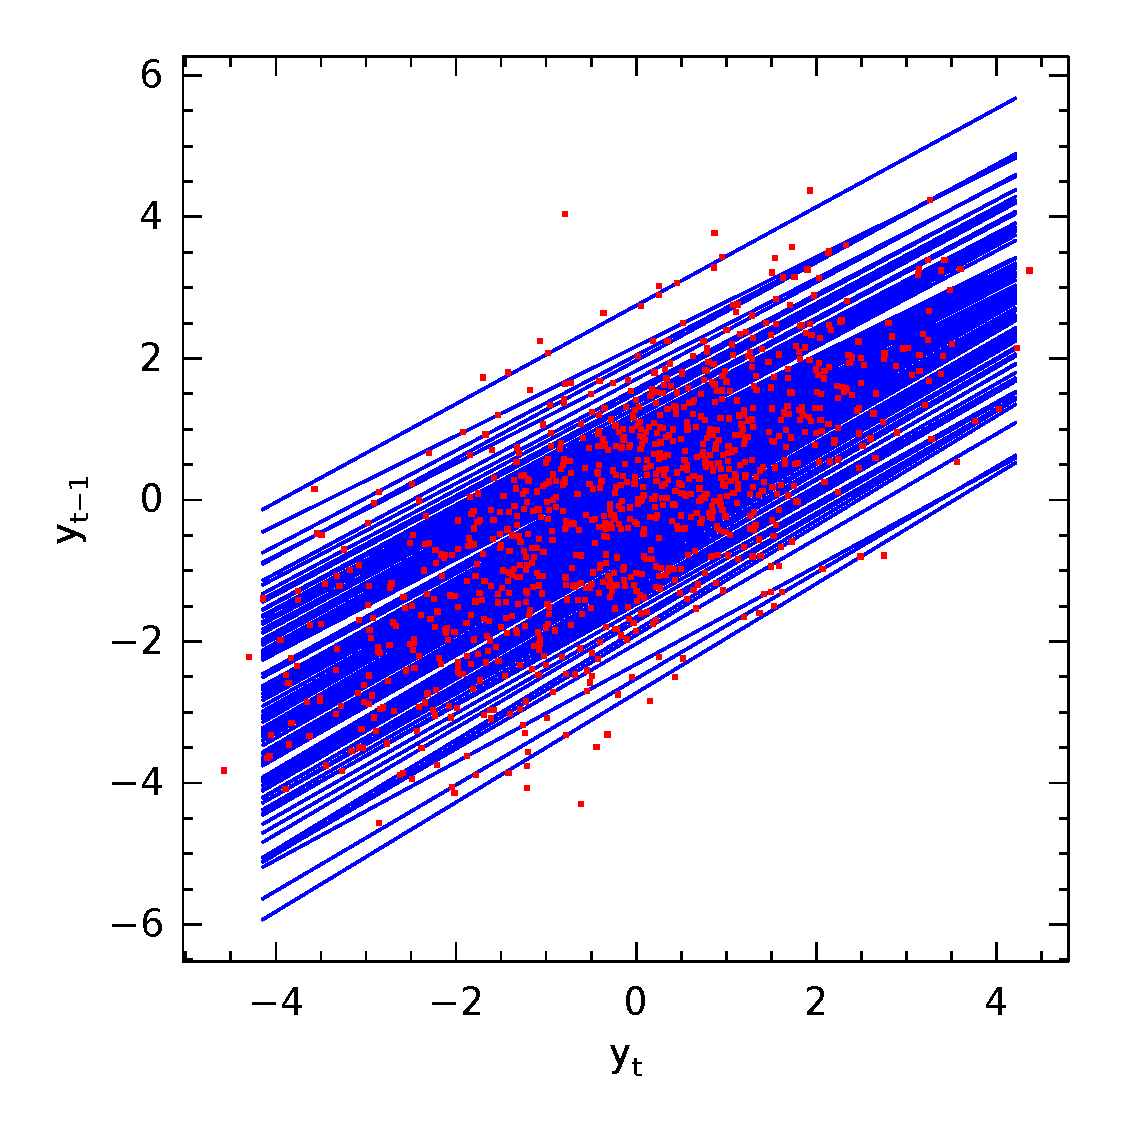
\includegraphics[width=0.5\linewidth]{Figuras/arima-crossing-10.pdf}
\caption{Dados simulados ARIMA com penalização $\lambda=10$}
\label{fig:arima-crossing-10}
\end{figure}

Na estimação com valor de $\lambda=0.3$ (figura \ref{fig:arima-crossing-03}), observamos que a estimação do quantil possui uma variância muito alta. Nesses casos, o erro \textit{in-sample} é baixo, mas as previsões serão muito ruins. À medida que o valor incrementamos o valor de $\lambda$ (figura \ref{fig:arima-crossing-1}, onde utilizamos $\lambda=1$), a função estimada para os quantis fica cada vez mais próxima de uma função linear, até que para valores mais extremos de $lambda$ (ver figura \ref{fig:arima-crossing-10}, onde utilizamos $\lambda=10$) ela será totalmente linear.

A restrição \ref{eq:non-crossing}, ao forçar que a função de nenhum quantil se cruze, produz uma diferença nos valores estimados. Esta diferença, no entanto, é perceptível apenas nas extremidades dos gráficos. As figuras \label{fig:arima-noncrossing-03} e \label{fig:arima-crossing-03} exemplificam as diferenças da inclusão ou não desta restrição.

%A seguir, apresentaremos alguns resultados para quando o 

%The difference between using or not this constraint can be seen in the two plots below:
%
%
%
%\bibliography{QR}
%\bibliographystyle{ieeetr}
%
%\end{document}